% !TEX program = arara
% arara: pdflatex
% arara: biber
% arara: pdflatex
% arara: pdflatex
% arara: clean: { files: [ Bericht.out ] }
% arara: clean: { files: [ Bericht.aux, Bericht.bbl ] }
% arara: clean: { files: [ Bericht.bcf, Bericht.blg ] }
% arara: clean: { files: [ Bericht.log, Bericht.run.xml ] }
% arara: clean: { files: [ Bericht.toc, Bericht-blx.bib ] }
% 

\documentclass{Bericht}
\usepackage{todonotes}
\usepackage[utf8]{inputenc}
\usepackage{hyperref} % http://ctan.org/pkg/hyperref
\usepackage{graphicx}
%\usepackage[ngerman]{babel} % deutsche Silbentrennung
\hypersetup{
	colorlinks = true,
	linkcolor  = black
}

\begin{document}

\maketitle

% % % % %

\tableofcontents
\clearpage

\section{Einleitung}
	\todo[inline]{Autor: Kim}

\section{Ideenfindung}
	\todo[inline]{Autor: Berna}
	Hier steht die Ideenfindung.

\section{Hypothese}
	\todo[inline]{Autor: Berna}
		Hier steht die Hypothese.

\clearpage
\section{Verlauf}
	\todo[inline]{Autor: Marvin \& Daniel}
	\subsection{Planung/Recherche} % Marvin
	
%Erster Kontakt
Erster Berührungspunkt mit dem Bachelorprojekt ¡Experiment! war für viele Gruppenmitglieder die Vorstellung eben dessen durch Thorsten Kluß am 24.01.2017 an der Hochschule für Künste, bzw. deren Wiederholung am 06.04.2017 an der Universität Bremen. Erweitert wurde der zweite Termin dabei durch eine Führung der Räume des 'Cartesiums', sowie eine Beschreibung der vorangegangen Bachelorprojekte. Hierdurch konnte ein erster Eindruck über die verschiedenen Versuchsaufbauten und ferner der Beschaffenheit unseres Projekts gewonnen werden. An dieser Stelle wurde zunächst eine Recherche-Aufgabe zu vorbereiteten Texten ausgeteilt, welche allein oder in kleineren Gruppen bearbeitet und später präsentiert werden sollte.\\
\\
%Erwartungen
Am darauffolgenden Termin wurden uns von den Dozenten (Thorsten Kluß und Jaime Maldonaldo, später zusätzlich Kerstin Bub) alle Erwartungen, sowie Schein- und Arbeitsbedingungen dargelegt.\\
\\
%Social & Arbeitsweise/Zeiten
Neben den üblichen 'Kennenlern-Ritualen', wie z.B. dem Herausstellen der eignen Stärken und Schwächen anhand von 'Skill-Profilen', wurden die ersten zwei Wochen der Projektarbeit hauptsächlich für technische Organisation, Planungs- und Recherchezwecke genutzt. Dabei entschied man zunächst, dass ein 'Scrum'-Modell mit geteilter 'Scrum-Master'-Position für das Projektmanagement genutzt werden soll. Anhand der bereits erwähnten Fähigkeitenprofile wurde die Gruppe 7-3 in zwei Teams mit unterschiedlichen Schwerpunkten aufgeteilt('Design' und 'Organisation').\\
Weiterhin wurde ein umfassender Stundenplan aus den einzelnen Stundenplänen für das restliche Studium jedes Teilnehmers erstellt. Anhand dessen wurden Zeiten an vier Tagen der Woche ermittelt, welche für Treffen der Arbeitsgruppe zum Bachelorprojekt genutzt werden sollten, mit einem zusätzlich Slot am Donnerstag für ein Meeting mit den Dozenten. \\
Zu Beginn jeden Arbeitstages wurde ein 10-minütiges 'Scrum-Treffen' gehalten, in denen anstehende Aufgaben aus dem Backlog und Probleme besprochen wurden. Diese besonderen Treffen wurden jedoch nie regelmäßig eingehalten, vor allem in späteren, arbeitsintensiveren Phasen nicht.\\
Ferner wurde für die Protokollführung der Treffen eine feste Reihenfolge angelegt.\\
\\
%Raum
Leider war es unseren Dozenten nicht möglich, eine dedizierten Raum für unseren Arbeitsprozesse zu erhalten, weshalb die Treffen je nach Situation im Konferenzraum [x.x] des vierten Stockwerks oder den Räumen [x.x] und [x.x](ebenfalls vierter Stock) im Cartesium abgehalten worden sind. Um Zugang zu der Etage und diesen Räumen zu gewährleisten, erhielten wir mit einiger Verzögerung jedoch Türchips für das spezielle Schließsystem des Cartesiums.\\
\\
% Tech
Auch wurden alle technischen Lösungen zur Arbeitsweise in dieser Zeit implementiert. Als zentrale Sammelstelle für sämtliche Dokumente wurde ein Board beim Service 'Trello' genutzt. Dort ließen sich bequem und zugänglich für alle Teilnehmer sämtliche wöchentlichen Sprints sowie der Backlog des Scrum, die Protokolle und der Stundenplan, etc. ablegen. Für schnelle Kommunikation untereinander wurde der Nachrichtendienst 'WhatsApp' genutzt, da diese Applikation bereits auf sämtlichen Endgeräten der Teilnehmer installiert war. Leider wurde dieser Dienst nicht von den Dozenten genutzt und wir verließen uns auf Kommunikation per E-Mail mit diesen, sowie Telefonate in dringenden Fällen.\\
\\
%Recherche
Die ersten Rechercheleistungen beschäftigten sich hauptsächlich mit wissenschaftlichen Arbeitsweisen, existierenden technischen Möglichkeiten und bereits durchgeführter Forschung. Vollkommen fehlgeleitet und geblendet von technischen Besonderheiten wie dem möglichen Hand-Tracking durch 'LeapMotion' oder der Bewegungsteuerung durch [die Kugel] versuchten wie eine Forschungsfrage passend zu diesen zu entwickeln.\\
Wie im 'Paragraphen 2: Ideenfindung' beschrieben, dauerte es eine gewisse Zeit bis wir eine konkrete, realisierbare Forschungsfrage zur Manipulation des Zeitempfindens innerhalb der 'Virtual Reality' ausarbeiten konnten. Maßgeblich geholfen hat uns dabei die Grundlagenforschung zur Zeitwahrnehmung in der VR von Gerd Bruder.\\
\\
%Überschneidung
Die genauen Spezifikationen an unser Experiment gemäß der Forschungsfrage wurden nach Rücksprache mit den Dozenten immer wieder verändert. Hierdurch entstand viel unbenutzbares Material, da wir überschneidend bereits damit begonnen hatten, 3D-Objekte nach den ersten Anforderungen für unsere Versuchswelt zu erstellen. Dies geschah fälschlicherweise aus dem Versuch heraus, bereits verlorene Zeit aufzuholen, wodurch jedoch nur mehr 'Verschnitt' produziert worden ist, was uns ultimativ uns mehr Zeit gekostet hat.\\
\\
%Weiterführend
Wir approximierten, dass sich ab diesem Zeitpunkt unser Projekt in 3 Phasen (Programmierphase, Versuchsphase, Evaluation/Paper) 	unterteilen ließe und legten Deadlines für die einzelnen fest. Im Laufe des Projektes sollten wir jedoch erkennen, wie weit entfernt diese Einschätzungen von der Realität abwichen.

	\subsection{Design} % Daniel
		\todo{methodisches Versuchsdesign}
		Angefangen haben wir mit dem Erstellen von 3D-Objekten. Aus einer Liste mit benötigten Objekten suchte sich jeder aus dem Technikteam einige heraus und begann sie zu designen. Folgende Objekte wurden erstellt, wenn auch nicht alle im finalen Projekt zum Einsatz kamen:
		
		\begin{itemize}
			\setlength{\itemsep}{0em}
			\item Ampel
			\item Autos
			\item Blume
			\item Bäume
			\item Büsche
			\item Garten
			\item Gehsteige
			\item Heißluftballon
			\item Hund
			\item Häuser
			\item Laterne
			\item Menschliche NPCs
			\item Mülleimer
			\item Parkbank
			\item Plakat
			\item Rasenfläche
			\item Reiher
			\item Schaukel
			\item Sonne
			\item Straße
			\item Straßenschilder
			\item Supermarkt
			\item Wolken
			\item Zimmerpflanze (Kaktus)
		\end{itemize}
		
		\begin{figure}[!htbp] % here - top - bottom - page, das ! erzwingt die Position falls möglich
			\centering
			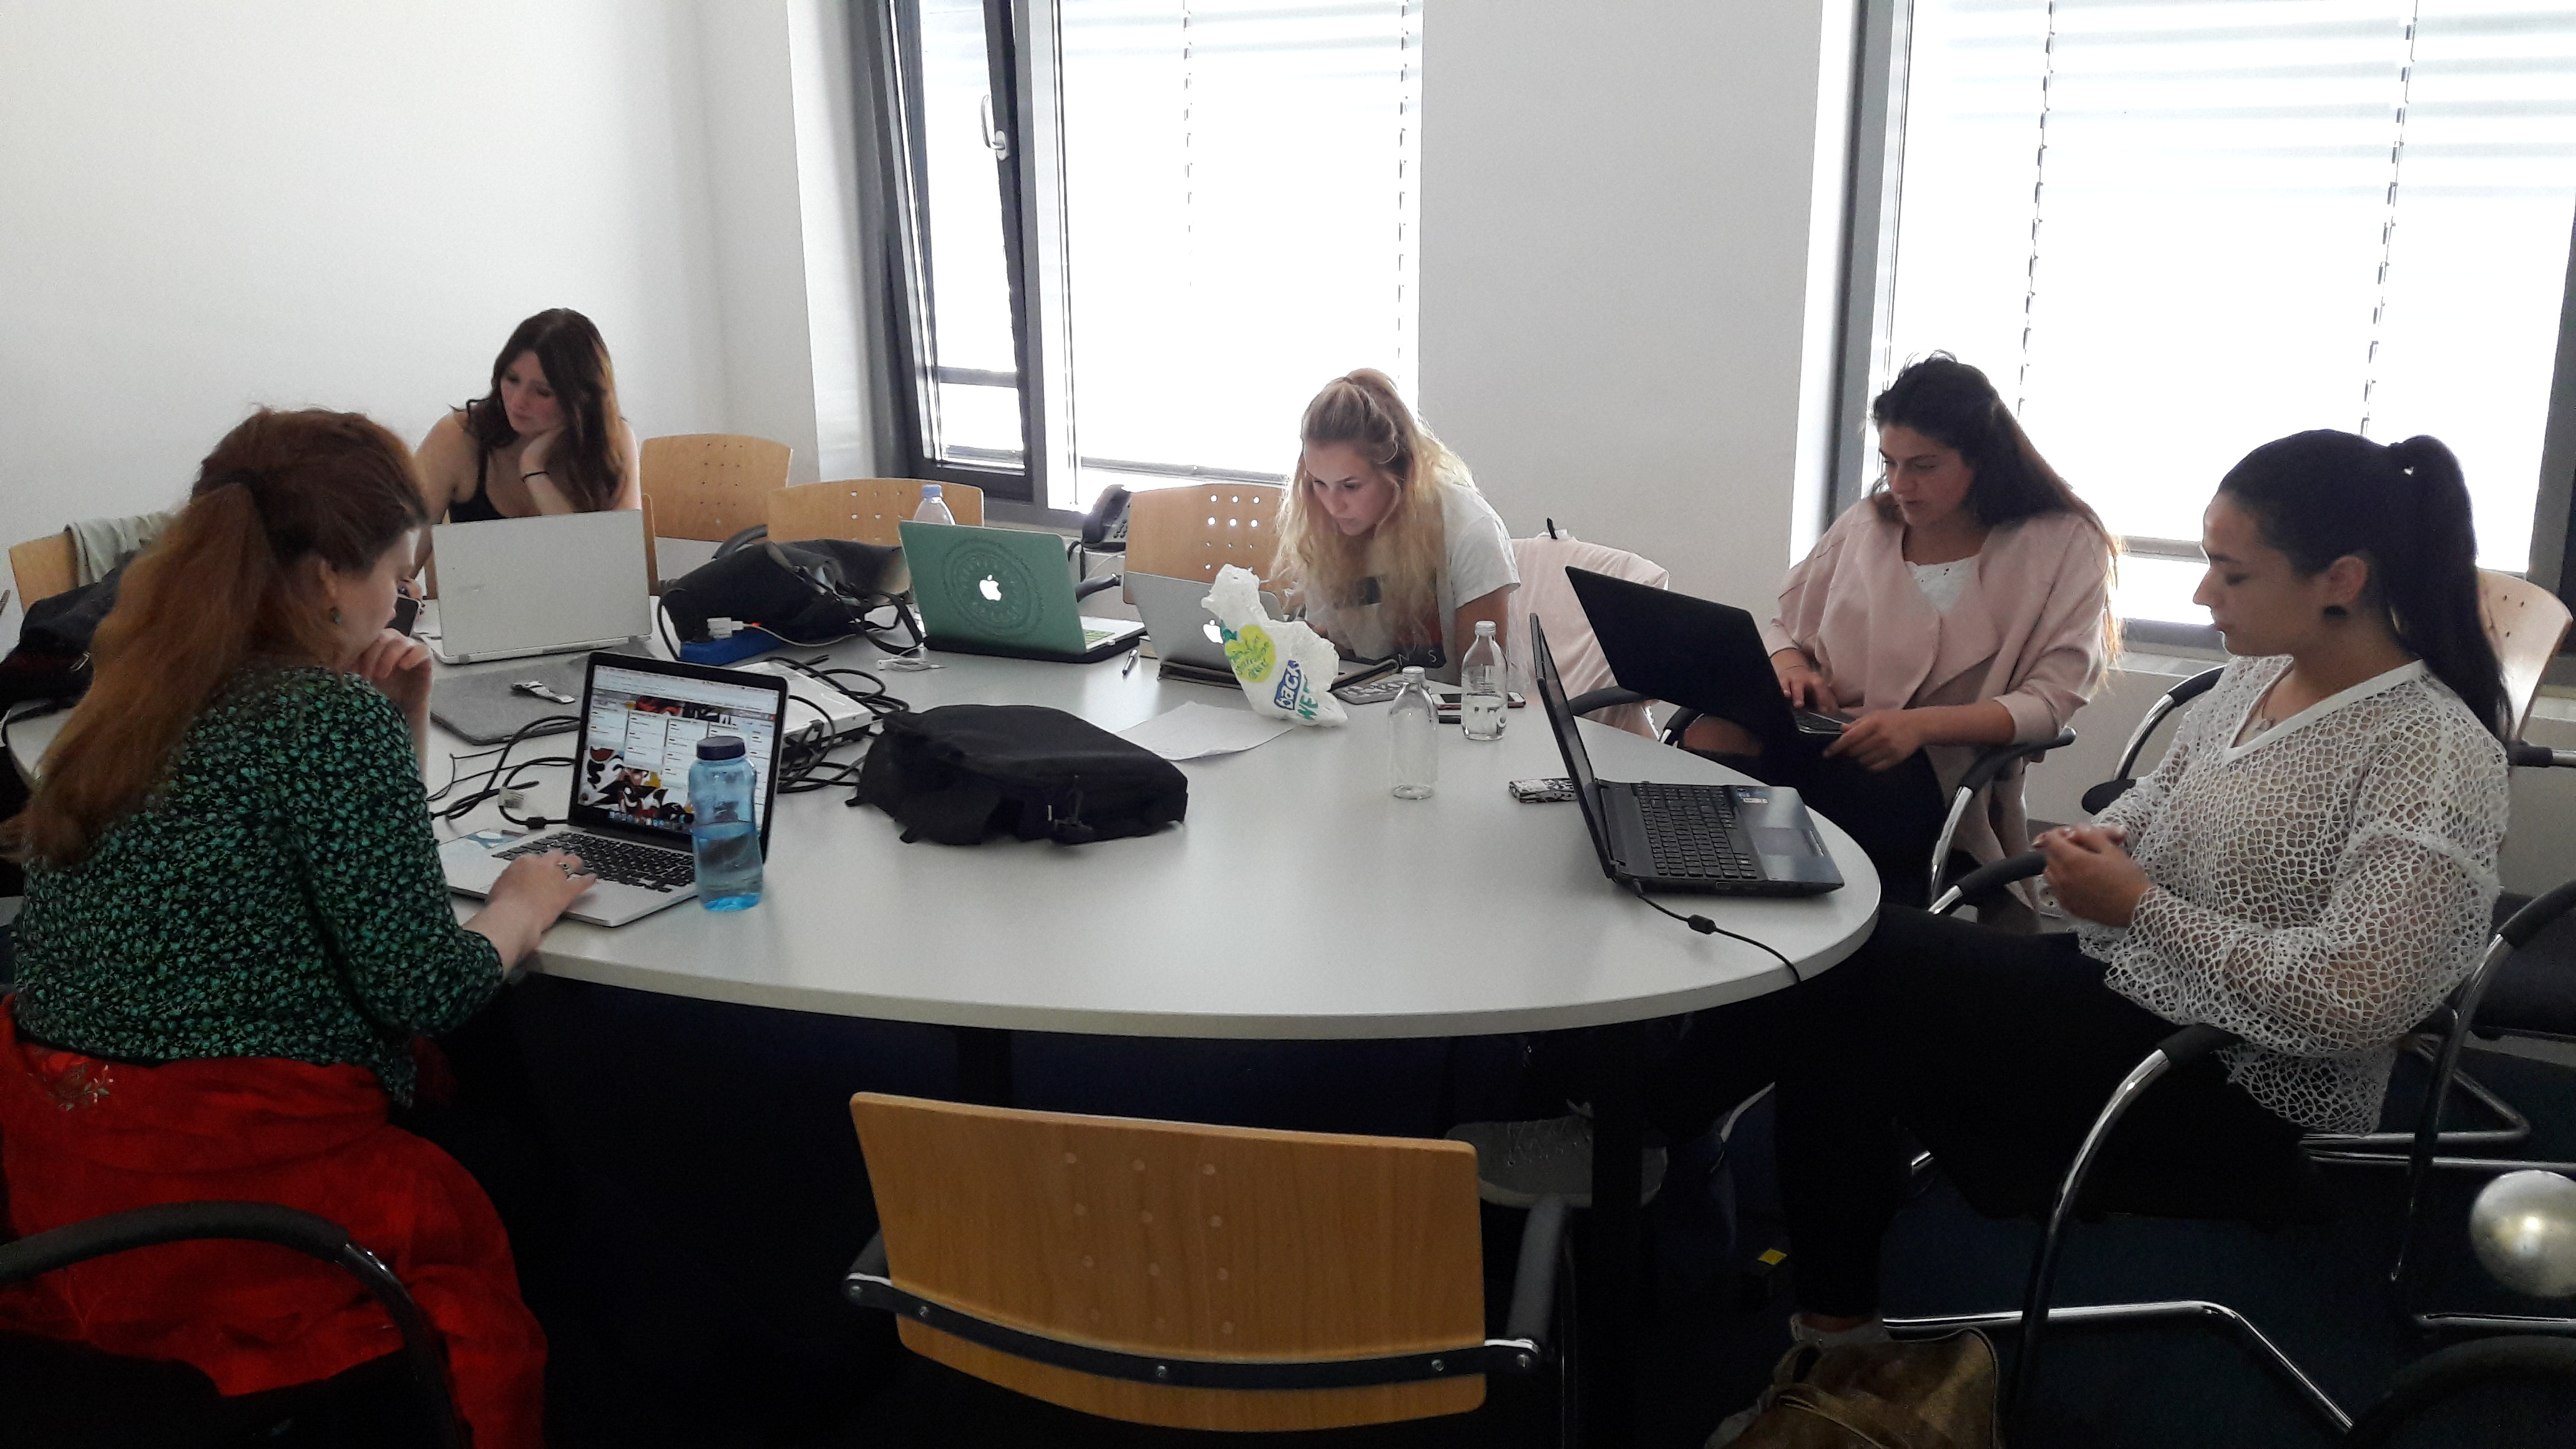
\includegraphics[width=\linewidth, height=\textheight, keepaspectratio]{Bilder/20170518_103125.jpg}
			\caption{Das ¡Experiment!-Team bei der Arbeit}
			\label{img:experiment-team-bei-der-arbeit}
		\end{figure}

		Die Welt war zuerst als recht große Welt geplant, in der man sich frei bewegen kann. Hier sollte man sich viele verschiedene interessante Dinge angucken können und frei durch die Gegend laufen. Hierbei stießen wir jedoch auf das Problem, dass verschiedene Versuchspersonen verschiedene Wege gehen würden und somit unterschiedliche Dinge erleben und manche Szenarien vielleicht sogar komplett auslassen würden. Um dies zu verhindern, kam uns die Idee eier Art Schnitzeljakt. Damit wäre gewährleistet gewesen, dass jeder Versuchsperson ungefähr die gleiche Strecke läuft und das gleiche erlebt wie alle anderen. Jedoch stellte sich auch das als nicht sehr praktikabel heraus. Wir benötigten ein Mapdesign, in dem jede Versuchsperson die gleiche Strecke läuft und das gleiche erlebt.

		So kamen wir darauf, die Versuchspersonen auf einem Gehweg entlanglaufen zu lassen, auf dem es keine betretbaren Abzweigungen gibt und jeder an mehreren Ampeln für eine vordefinierte Zeit warten muss. 
		
		Während des gesamten Designprozesses kam es immer wieder zu Schwierigkeiten und Problemen.
		
		\subsubsection{Blender}
			Blender ist ein sehr komplexes und umfangreiches Programm, dementsprechend hatte jeder von uns eine längere Einarbeitungsphase. Bei kleineren Problemen haben wir uns gegenseitig viel helfen können und unser angesammeltes Wissen ausgetauscht. Die größten Probleme entstanden hauptsächlich nach dem Import in die Unreal Engine. 
%			Normale
%			Texturen
			
			Ein zentrales Problem war, dass jegliche von uns erstellten Objekte nach eine Build des Lightnings komplett schwarz waren. Nach einiger Recherche stellte sich heraus, dass alle in der Unreal Engine verwendeten Objekte zwei UV-Maps benötigen. Die zweite ist notwendig für das korrekte Darstellen des Lightning und ist, zumindest bei statischen Objekten, zwingend notwendig. Sich bewegende Objekte wie beispielsweise die Autos werden anders gerendert und benötigen diese zweite UV-Map nicht. 
		
		\subsubsection{Unreal}
		
		\subsubsection{Hardware}
		
%		Probleme
%			Blender
%			Unreal
%			Controler
%			Kugel
%			Oculus
%			PC-Wechsel
%			Fahrrad
%			Teleport

	\subsection{Versuchsdurchführung} % Daniel
	\subsection{Auswertung} % Marvin
	
%Auswertung
Das Projekt abschließend folgte nach dem 26.03.2017, dem letzten Tag der Versuchsdurchführung, die Auswertung unserer Ergebnisse.
Zunächst mussten wir auch in dieser Phase einige zusätzliche Recherche, vor allem zu mathematischen Verfahren für statistische Auswertung, betreiben. Ebenfalls sehr wichtig waren für uns die genauen Richtlinien zur Veröffentlichung eines wissenschaftlichen Papers. Hierzu erhalten wir ein maßgebendes Buch von unseren Dozenten. Wir unterteilten den Inhalt des Papers und dieses Berichts und teilten diese untereinander auf.\\
Danach begannen wir zunächst damit sämtliche Ergebnisse zu digitalisieren.\\
\\

\section{Versuchsaufbau und Durchführung}
	\todo[inline]{Autor: Nizan}
	\subsection{Probanden}
	\subsection{Aufbau \& Apparaturen}
	\subsection{Experiment Ablauf}
	\subsubsection{Fragebögen}
	\subsubsection{Intelligenztest}
	\subsubsection{Genaue Wortlaute bei der Testphase}
	\subsubsection{Schwierigkeiten}
	\subsection{Ethik}

\section{Beobachtungen}
	\todo[inline]{Autor: Nicole \& Svenja}
	Nur Verweis auf Paper!

\section{Auswertung}
	\todo[inline]{Autor: Nicole \& Svenja}
	Nur Verweis auf Paper!

\section{Interpretation}
	\todo[inline]{Autor: Nicole \& Svenja}
	Nur Verweis auf Paper!
	
\section{Fazit}
	\todo[inline]{Autor: Chovi}

	Zusammenfassung: Was wurde grob in dieser Arbeit gemacht? Was waren die Schlüsselergebnisse?

	Wem nützen die Beiträge der Arbeit? Inwieweit wird die Wissenschaft durch die Arbeit verbessert?

	Aufbauende Arbeiten: Welche möglichen Lösungsansätze für noch bestehende Probleme sind denkbar(mehr Probanden)? Wie könnten Folgearbeiten aussehen?

\section{Abschließende Gedanken}
	\todo[inline]{Autor: Jana}
	Wir sind in den verschiedenen Phasen des Projekts auf unterschiedliche Probleme gestoßen, von denen wir viele zeitnah lösen konnten. Allerdings gab es auch schwerwiegendere, deren Lösung für uns nicht gleich oder gar nicht offensichtlich war und die unseren ursprünglichen Zeitplan infolgedessen ungewollt stark beeinflusst haben.\\
	Eines der größten Hindernisse in unserem Projekt waren technische Probleme, die ein Vorankommen sehr stark verzögerten und in einem veränderten Zeitplan resultierten.\\
	Durch die Inkompabilität der Ocolus Rift und dem Computer der Virtusphere konnten wir unser Projekt nicht wie ursprünglich geplant in der Virtusphere stattfinden lassen und mussten auf herkömmliche Controller ausweichen. Diese Umstellung ist sehr ärgerlich, da viel Zeit in die Problemlösung investiert wurde und wir den Probanden letztendlich doch nicht das bieten konnten, mit dem wir sie ursprünglich geworben haben. 
	Weiterhin zu kritisieren wäre eine nicht ganz ideale Arbeitsteilung, wodurch es gerade am Ende zu erheblichem Zeitverzug kam. Insbesondere das sog. \textit{Technikteam}, welches primär für die Erstellung der Blenderobjekte, das Einsetzen und das Animieren der Welt verantwortlich war, hat gleich zu Beginn des Projekts anstehende Aufgaben nicht sinnvoll verteilt. Alle Mitglieder waren gleichermaßen nur mit \textit{aktuellen} Aufgaben beschäftigt. D.h., dass zunächst alle für die Erstellung von Blenderobjekten verantwortlich waren und so Kapazitäten und Zeit verschwendet wurde, da sich bisher noch keiner besonders gut mit der Software auskannte und sich alle gleichermaßen neu einarbeiten mussten.\\
	Diese Entscheidung mag daraus resultieren, dass wir im Bezug auf so eine Art von selbstorganisierter Arbeit sehr unerfahren sind und es dadurch zu Fehleinschätzungen kam.\\
	Im Nachhinein stellen wir weiterhin fest, dass es für das Projekt besser gewesen wäre, hätten wir zu Beginn andere Prioritäten festgelegt. Da die Logik der Welt der Punkt ist, von dem die Ergebnisse abhängen, hätte man sich zuallererst auch mit dieser beschäftigen müssen bzw. rechtzeitig die Personen bestimmen müssen, die die Hauptverantwortung für diese übernehmen.\\
	Auch diese Fehleinschätzung zeigte sich im Nachhinein als kritisch.

\section{Appendix} % = Anhang
	\todo[inline]{Autor: Alina}
	Anhang.
	
\vfill %Zum Seitenende Verschieben

\printbibliography

\end{document}
